\chapter{Questionnaire statistics}
\label{app:questionnaire}

\FloatBarrier
\section{Descriptives of Perceived Usefulness questions}

\begin{longtable}[c]{@{}lrrrrrrrrrr@{}}
\caption{Flashcard condition}
\endfirsthead
\endhead
\toprule\addlinespace
& N & min & max & mean & variance & skew & kurt & norm-t &
norm-p & $\alpha$
\\\addlinespace
\midrule
\textbf{ctt} & 12 & -4 & 14 & 6.50 & 27.36 & -0.57 & -0.52 & 1.144 &
0.5643 & 0.6432
\\\addlinespace
\textbf{irt} & 12 & -5 & 1 & -0.16 & 4.40 & -1.89 & 3.15 & 17.284 &
0.0002 & 0.6263
\\\addlinespace
\bottomrule
    \label{tab:usefulness_fc}
\end{longtable}

\begin{figure}
    \centering
    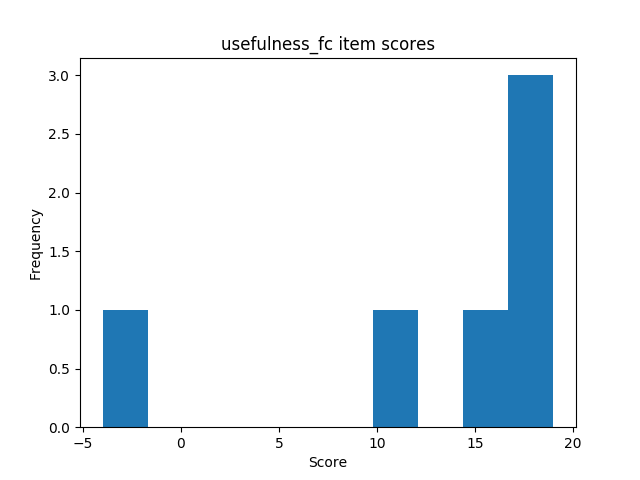
\includegraphics[width=.7\textwidth]{img/usefulness_fc_diff.png}
    \caption{A histogram depicting the scores per Perceived Usefulness item by flashcard users}
    \label{fig:usefulness_fc_diff}
\end{figure}
\begin{figure}
    \centering
    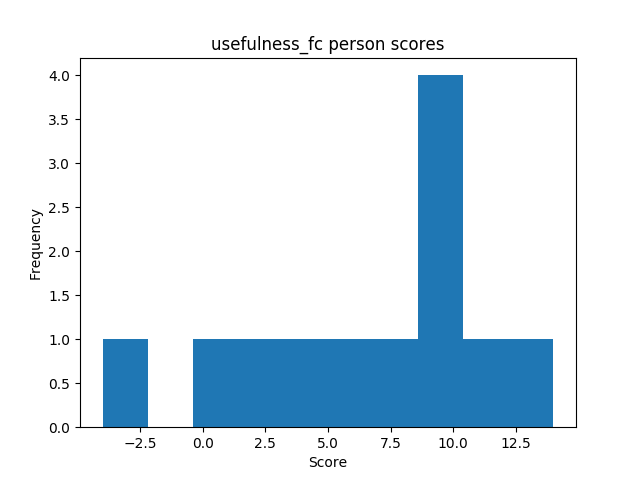
\includegraphics[width=.7\textwidth]{img/usefulness_fc_abil.png}
    \caption{A histogram depicting the scores on the Perceived Usefulness items per flashcard user}
    \label{fig:usefulness_fc_abil}
\end{figure}

\begin{longtable}[c]{@{}lrrrrrrrrrr@{}}
\caption{Flashmap condition}
\endfirsthead
\toprule\addlinespace
& N & min & max & mean & variance & skew & kurt & norm-t &
norm-p & $\alpha$
\\\addlinespace
\midrule
\textbf{ctt} & 11 & 0 & 13 & 8.82 & 15.16 & -1.05 & 0.32 & 4.698 &
0.0955 & 0.6777
\\\addlinespace
\textbf{irt} & 11 & -3 & 1 & -0.15 & 1.89 & -1.41 & 1.44 & 9.670 &
0.0079 & 0.5298
\\\addlinespace
\bottomrule
    \label{tab:usefulness_fm}
\end{longtable}

\begin{figure}
    \centering
    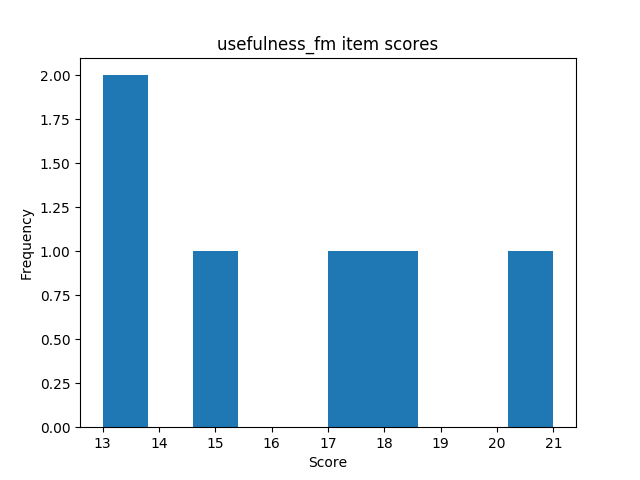
\includegraphics[width=.7\textwidth]{img/usefulness_fm_diff.png}
    \caption{A histogram depicting the scores per Perceived Usefulness item by flashmap users}
    \label{fig:usefulness_fm_diff}
\end{figure}
\begin{figure}
    \centering
    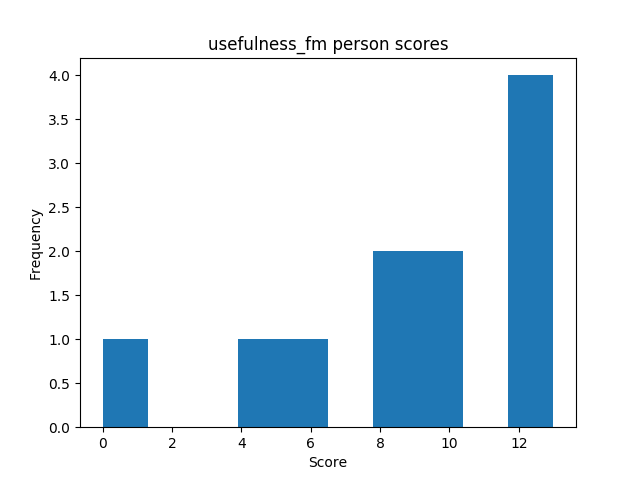
\includegraphics[width=.7\textwidth]{img/usefulness_fm_abil.png}
    \caption{A histogram depicting the scores on the Perceived Usefulness items per flashmap user}
    \label{fig:usefulness_fm_abil}
\end{figure}

\begin{longtable}[c]{@{}lrrrrrrrrrr@{}}
\caption{Combined conditions}
\endfirsthead
\toprule\addlinespace
& N & min & max & mean & variance & skew & kurt & norm-t &
norm-p & $\alpha$
\\\addlinespace
\midrule
\textbf{ctt} & 23 & -4 & 14 & 7.61 & 21.98 & -0.86 & -0.02 & 3.864 &
0.1448 & 0.6509
\\\addlinespace
\textbf{irt} & 23 & -3 & 2 & 0.49 & 1.82 & -0.73 & 0.55 & 4.058 & 0.1315
& 0.4619
\\\addlinespace
\bottomrule
    \label{tab:usefulness_gen}
\end{longtable}

\begin{figure}
    \centering
    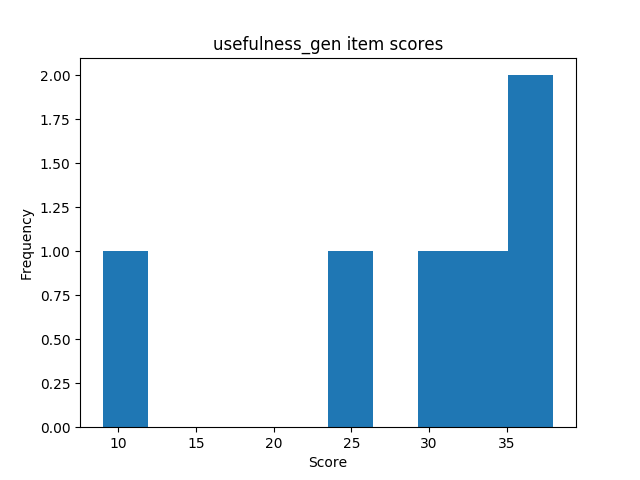
\includegraphics[width=.7\textwidth]{img/usefulness_gen_diff.png}
    \caption{A histogram depicting the scores per Perceived Usefulness item}
    \label{fig:usefulness_gen_diff}
\end{figure}
\begin{figure}
    \centering
    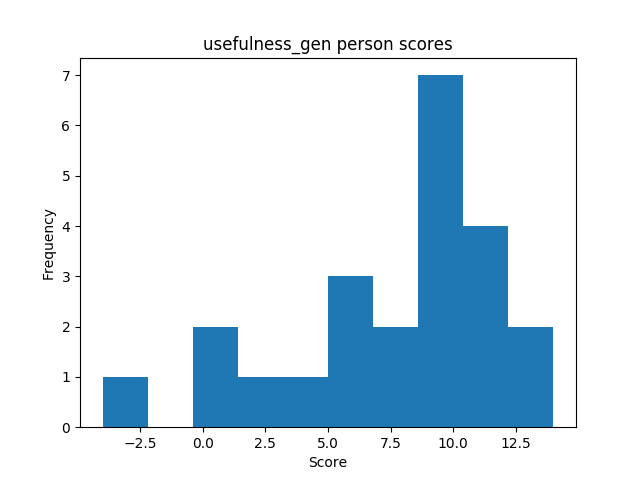
\includegraphics[width=.7\textwidth]{img/usefulness_gen_abil.png}
    \caption{A histogram depicting the scores on the Perceived Usefulness items per user}
    \label{fig:usefulness_gen_abil}
\end{figure}

\FloatBarrier
\section{Descriptives of Perceived Ease of Use questions}\label{ease-of-use}

\begin{longtable}[c]{@{}lrrrrrrrrrr@{}}
\caption{Flashcard condition}
\endfirsthead
\toprule\addlinespace
& N & min & max & mean & variance & skew & kurt & norm-t &
norm-p & $\alpha$
\\\addlinespace
\midrule
\textbf{ctt} & 12 & -4 & 17 & 6.58 & 38.08 & -0.26 & -0.62 & 0.232 &
0.8904 & 0.8794
\\\addlinespace
\textbf{irt} & 12 & 0 & 4 & 0.91 & 1.87 & 1.08 & 0.52 & 5.358 & 0.0686 &
0.2295
\\\addlinespace
\bottomrule
    \label{tab:easeofuse_fc}
\end{longtable}

\begin{figure}
    \centering
    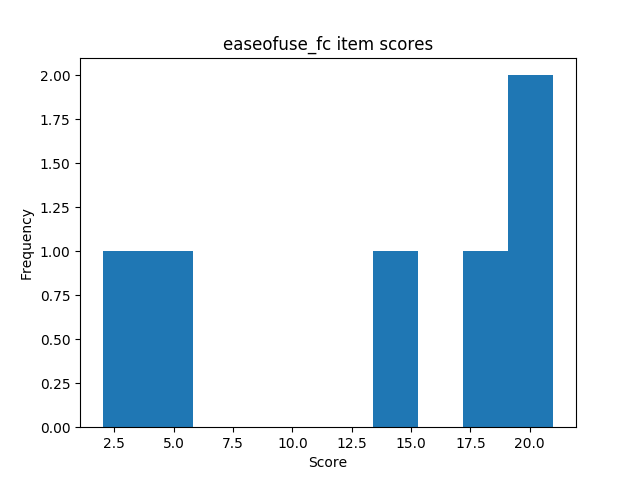
\includegraphics[width=.7\textwidth]{img/easeofuse_fc_diff.png}
    \caption{A histogram depicting the scores per Perceived Ease of use item by flashcard users}
    \label{fig:easeofuse_fc_diff}
\end{figure}
\begin{figure}
    \centering
    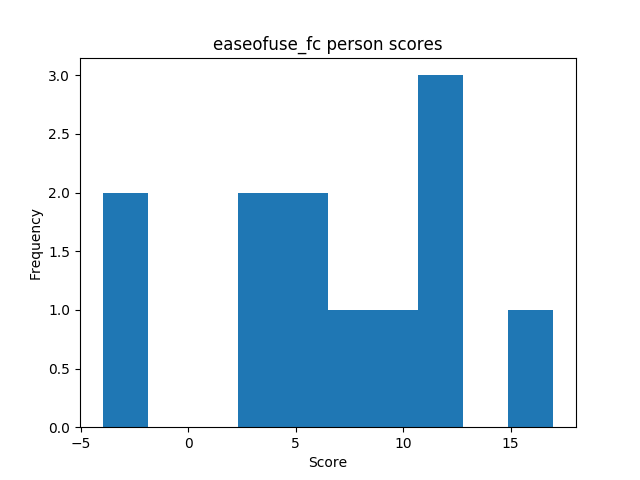
\includegraphics[width=.7\textwidth]{img/easeofuse_fc_abil.png}
    \caption{A histogram depicting the scores on the Perceived Ease of use items per flashcard user}
    \label{fig:easeofuse_fc_abil}
\end{figure}

\begin{longtable}[c]{@{}lrrrrrrrrrr@{}}
\caption{Flashmap condition}
\endfirsthead
\toprule\addlinespace
& N & min & max & mean & variance & skew & kurt & norm-t &
norm-p & $\alpha$
\\\addlinespace
\midrule
\textbf{ctt} & 11 & 0 & 19 & 8.27 & 26.22 & 0.50 & 0.12 & 1.725 & 0.4220
& 0.7689
\\\addlinespace
\textbf{irt} & 11 & -2 & 2 & 0.22 & 1.87 & -0.20 & 1.01 & 3.041 & 0.2186
& 0.2538
\\\addlinespace
\bottomrule
    \label{tab:easeofuse_fm}
\end{longtable}

\begin{figure}
    \centering
    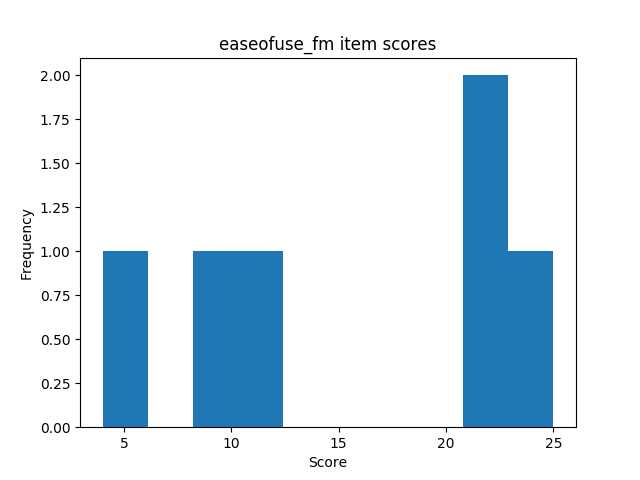
\includegraphics[width=.7\textwidth]{img/easeofuse_fm_diff.png}
    \caption{A histogram depicting the scores per Perceived Ease of use item by flashmap users}
    \label{fig:easeofuse_fm_diff}
\end{figure}
\begin{figure}
    \centering
    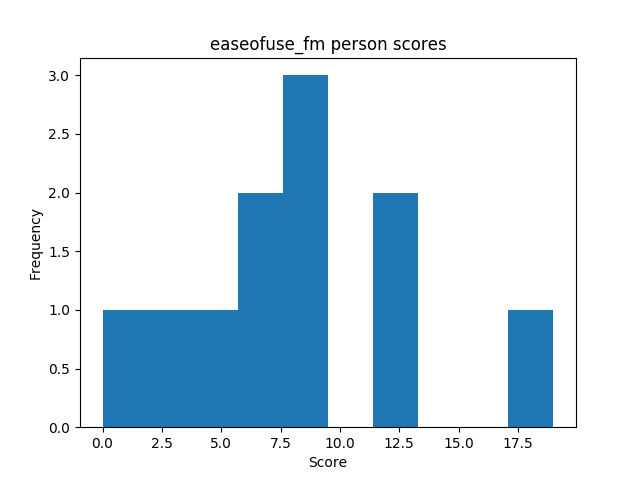
\includegraphics[width=.7\textwidth]{img/easeofuse_fm_abil.png}
    \caption{A histogram depicting the scores on the Perceived Ease of use items per flashmap user}
    \label{fig:easeofuse_fm_abil}
\end{figure}

\begin{longtable}[c]{@{}lrrrrrrrrrr@{}}
\caption{Combined conditions}
\endfirsthead
\toprule\addlinespace
& N & min & max & mean & variance & skew & kurt & norm-t &
norm-p & $\alpha$
\\\addlinespace
\midrule
\textbf{ctt} & 23 & -4 & 19 & 7.39 & 31.70 & -0.08 & -0.10 & 0.239 &
0.8876 & 0.8285
\\\addlinespace
\bottomrule
    \label{tab:easeofuse_gen}
\end{longtable}

\begin{figure}
    \centering
    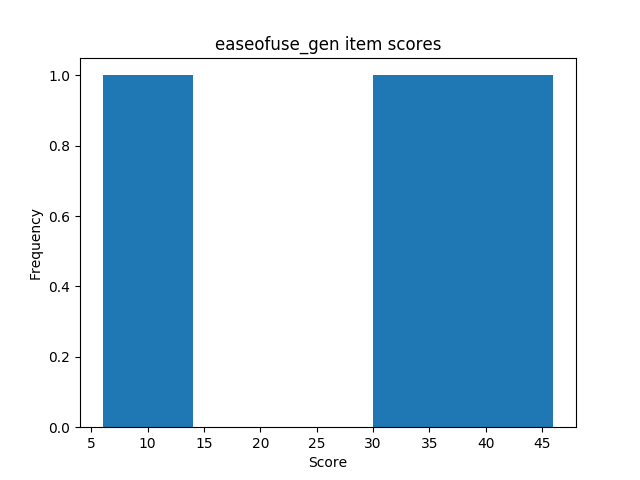
\includegraphics[width=.7\textwidth]{img/easeofuse_gen_diff.png}
    \caption{A histogram depicting the scores per Perceived Ease of use item}
    \label{fig:easeofuse_gen_diff}
\end{figure}
\begin{figure}
    \centering
    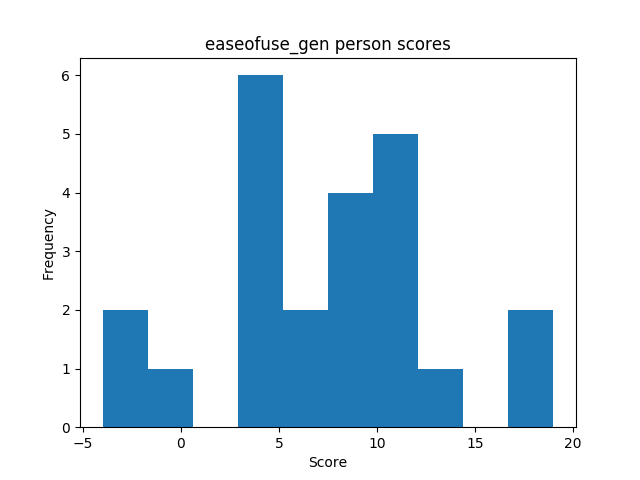
\includegraphics[width=.7\textwidth]{img/easeofuse_gen_abil.png}
    \caption{A histogram depicting the scores on the Perceived Ease of use items per user}
    \label{fig:easeofuse_gen_abil}
\end{figure}

\FloatBarrier
\section{Comparisons of the Perceived Usefulness questions}


\begin{longtable}[c]{@{}lrrrr@{}}
\toprule\addlinespace
& \textbf{MW k} & \textbf{MW p} &
\textbf{t-test k} & \textbf{t-test p}
\\\addlinespace
\midrule
\textbf{ctt} & -1.196 & 0.2449 & -1.212 & 0.2395
\\\addlinespace
\textbf{irt} & -0.014 & 0.9891 & -0.014 & 0.9889
\\\addlinespace
\bottomrule
    \label{tab:usefulness_comp}
\end{longtable}

\begin{figure}
    \centering
    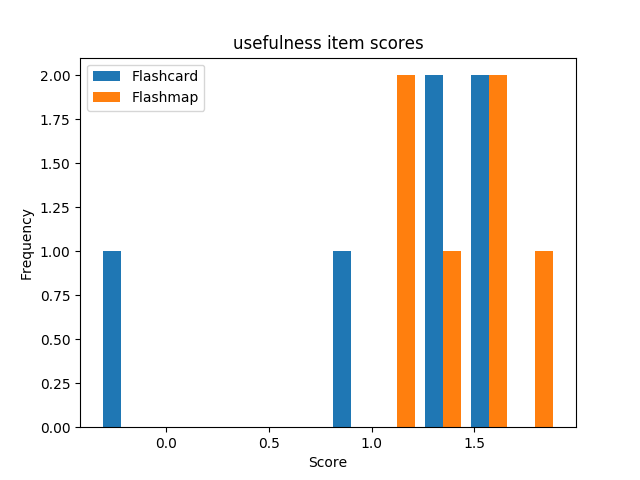
\includegraphics[width=.7\textwidth]{img/usefulness_diff.png}
    \caption{A comparison of figure~\protect\ref{fig:usefulness_fc_diff} and~\protect\ref{fig:usefulness_fm_diff}}
    \label{fig:usefulness_diff}
\end{figure}
\begin{figure}
    \centering
    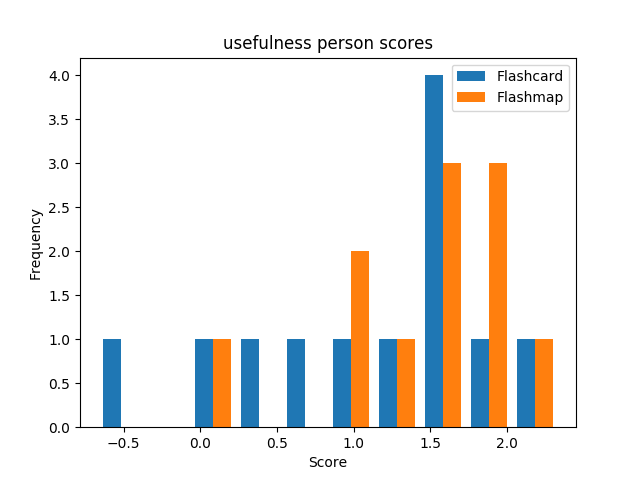
\includegraphics[width=.7\textwidth]{img/usefulness_abil.png}
    \caption{A comparison of figure~\protect\ref{fig:usefulness_fc_abil} and~\protect\ref{fig:usefulness_fm_abil}}
    \label{fig:usefulness_abil}
\end{figure}

\FloatBarrier
\section{Comparisons of the Perceived Usefulness questions}

\begin{longtable}[c]{@{}lrrrr@{}}
\toprule\addlinespace
& \textbf{MW k} & \textbf{MW p} &
\textbf{t-test k} & \textbf{t-test p}
\\\addlinespace
\midrule
\textbf{ctt} & -0.711 & 0.4851 & -0.717 & 0.4816
\\\addlinespace
\textbf{irt} & 1.206 & 0.2411 & 1.206 & 0.2412
\\\addlinespace
\bottomrule
    \label{tab:easeofuse_comp}
\end{longtable}

\begin{figure}
    \centering
    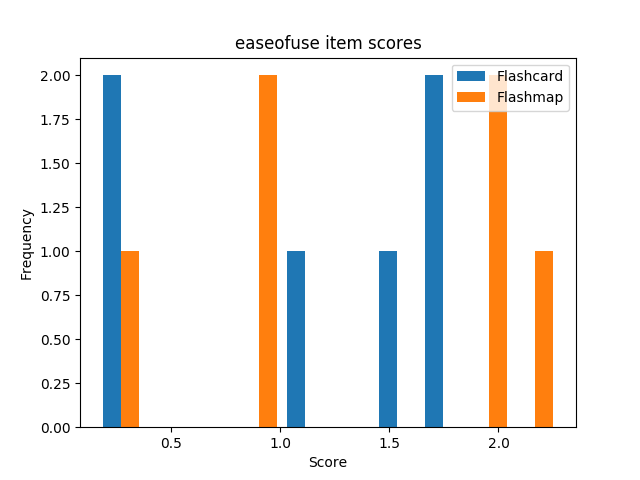
\includegraphics[width=.7\textwidth]{img/easeofuse_diff.png}
    \caption{A comparison of figure~\protect\ref{fig:easeofuse_fc_diff} and~\protect\ref{fig:easeofuse_fm_diff}}
    \label{fig:easeofuse_diff}
\end{figure}
\begin{figure}
    \centering
    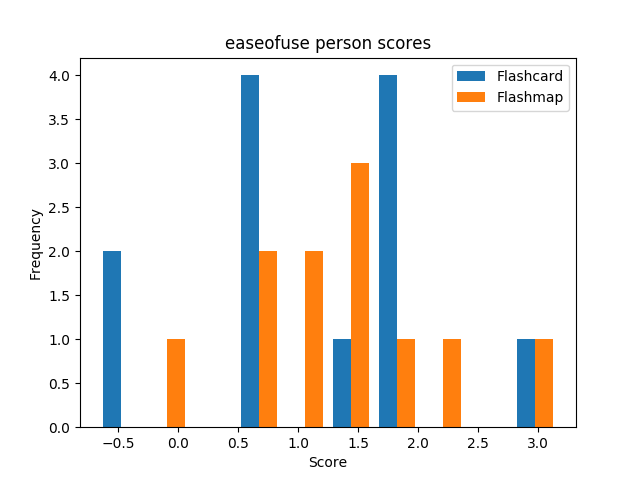
\includegraphics[width=.7\textwidth]{img/easeofuse_abil.png}
    \caption{A comparison of figure~\protect\ref{fig:easeofuse_fc_abil} and~\protect\ref{fig:easeofuse_fm_abil}}
    \label{fig:easeofuse_abil}
\end{figure}
